\documentclass{article}
\usepackage{url}
\usepackage{pgf}
\usepackage{listings}
\setlength{\parindent}{0pt}
\newtheorem{figcaption}[figure]{Figure}


\title{Beast II SDK: version 0.1}

%\subtitle{}

\author{Remco R. Bouckaert\\\url{remco@cs.{auckland|waikato}.ac.nz}\\
  Department of Computer Science\\
  University of Auckland \& University of Waikato
}

\begin{document}
\maketitle
\begin{abstract}
This is a short description of the Beast II Software Development Kit,
which includes a Java library for building Markov Chain Monte Carlo (MCMC) 
applications using the Metropolis Hastings method and a library for
Bayesian analysis of evolutionary problems.

In particular, there is support for efficient updating of models,
GUIs for building models and support for documentation. Newly written Plugins 
will be directly available in the GUIs, online help and HTML documentation.
\end{abstract}


\section{Introduction}

Beast II is written in Java, open source and licensed under the Lesser GNU Public License.
The Beast II SDK can be downloaded from \url{http://code.google.com/p/beast2/downloads/list}
and the source is available from \url{http://code.google.com/p/beast2/source/checkout}.

Beast II typically runs as a standalone application, started from the command line with
{\tt java -jar beast.jar} which starts {\tt beast.app.BeastMCMC}.
An XML file should be specified as command line argument. XML files are used to
store models and data in a single place. See Section \ref{sec.xml} for details.

To use the SDK, you write Java classes that derive from the {\tt Plugin} class, or derive
from any of the more specialized classes that derive from {\tt Plugin}. By default,
the classes are expected to reside in a jar file in the {\tt beastlib} directory
from where BeastMCMC (or any of the other applications) is started. To specify another
locations, either set the {\tt beastlib} environment variable to the directory (or
directories where the various directories are separated by a colon, just like in Java
class paths) where the jar file should be picked up.


\section{Example\label{sec.example}}

%\begin{figure*}[h]
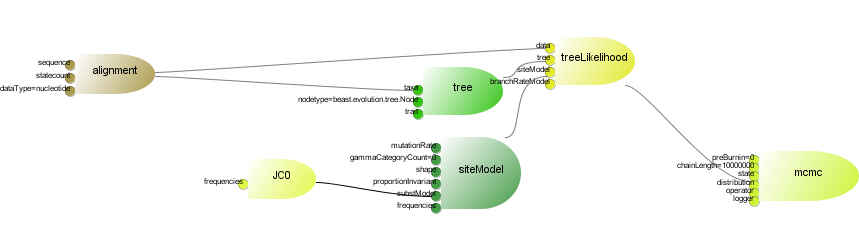
\includegraphics[width=\textwidth]{example1.png}
\figcaption{\label{fig.jc}Example of a model specifying Jukes Cantors substriution model (JC).
It shows Plugins represented by rocket shapes connected to other Plugins through inputs 
(the thrusters of the rocket).}\rm\\\hskip10pt
%\end{figure*}

Figure \ref{fig.jc} show (part of) a model, representing an nucleotide sequence analysis 
using the Jukes Cantor substitution model. The 'rockets' represent plugins, and their
thrusters the inputs. Models can be build up by connecting plugins through these inputs
with other plugins. For example, in Figure \ref{fig.jc}, the Tree has an Alignment
as input, and both Tree and Alignment are inputs to the TreeLikelihood. The TreeLikelihood
calculates the likelihood of the sequence for a given tree. To do this, the TreeLikelihood
also needs at least a SiteModel as input, and potentially also a BranchRateModel (not
necessary in this example). The SiteModel specifies everything related to the transition
probabilities for a site from one node to another in the Tree, such as the number of
gamma categories, proportion of invariant sites and substitution model. In Figure \ref{fig.jc},
Jukes Cantor substitution model is used. In this Section,  we extend this with the 
HKY substitution model and show how this model interacts with the operators,
state, loggers and other bits and pieces in the model.


%\begin{figure*}[h]
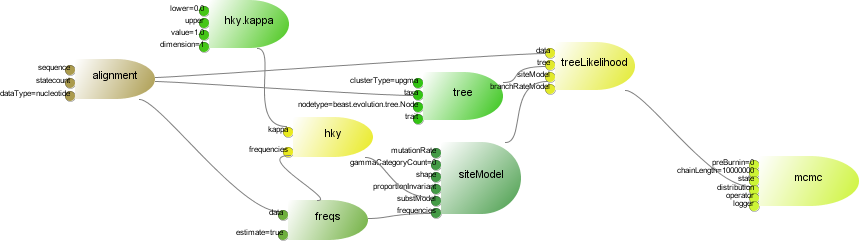
\includegraphics[width=\textwidth]{example2.png}
\figcaption{\label{fig.hky}Example of a model specifying a HKY substitution model.}\rm\\\hskip10pt
%\end{figure*}

To define the HKY substitution model, first we need to find out what its inputs should be.
The kappa parameter of the HKY model represents a variable that can be estimated.
Plugins in the calculation model (i.e. the part of the model that performs the posterior
calculation) are divided in StateNodes and CalculationNodes. StateNodes are classes
an operator can change, while CalculationNodes are classes that change the internal
state based on Inputs. 
The HKY model is a CalculationNode, since it internally stores an eigenvalue 
matrix that is calculated based on kappa. Kappa can be changed by an operator and does
not calculate antying itself, so the kappa parameter is a StateNode.

The other bit of information required for the HKY model it the character frequencies.
These can be calculated from the alignment.%, so Frequencies is a CalculationNode. <- NOT CORRECT
Compare Figure \ref{fig.hky} with Figure \ref{fig.jc} to see how the HKY model differs
from the JC model.
See Section \ref{sec.start} for implementation details for plugin classes like HKY.


%\begin{figure*}[h]
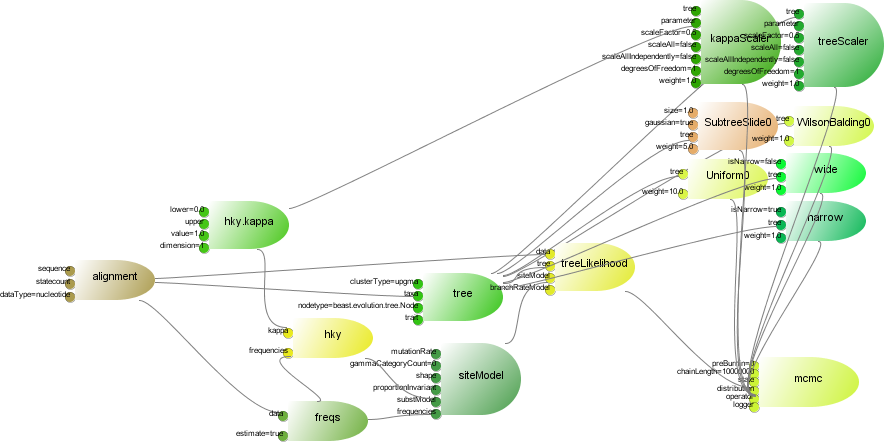
\includegraphics[width=\textwidth]{example3.png}
\figcaption{\label{fig.hky2}Adding operators.}\rm\\\hskip10pt
%\end{figure*}

In an MCMC framework, operators propose a move in the state space, and these are
then accepted or rejected based on how good the moves are and luck. Figure \ref{fig.hky2}
shows the HKY model extended with seven operators: six for changing the tree and
one for changing the kappa parameter.


%\begin{figure*}[h]
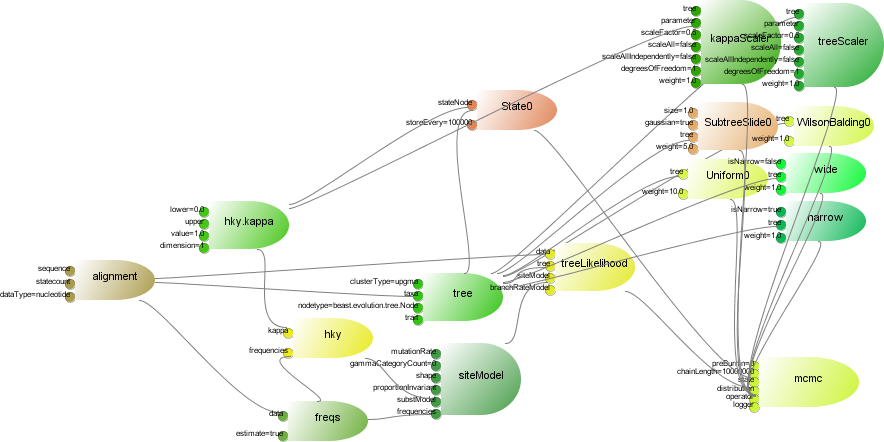
\includegraphics[width=\textwidth]{example4.png}
\figcaption{\label{fig.hky3}Adding the state.}\rm\\\hskip10pt
%\end{figure*}


The operators work on the tree and the kappa parameter. Any StateNode that an operator
can work on must be part of the State. Apart from the State being a collection of
StateNodes, the State performs introspection on the model and controls the order in
which Plugins are notified of changes and which of them should store or restore their
internal state. For example, if an operator changes the Tree, the HKY model does not
need to be bothered with updating its internal state or storing that internal state
since it never needs to be restored based on the tree change alone.

%\begin{figure*}[h]
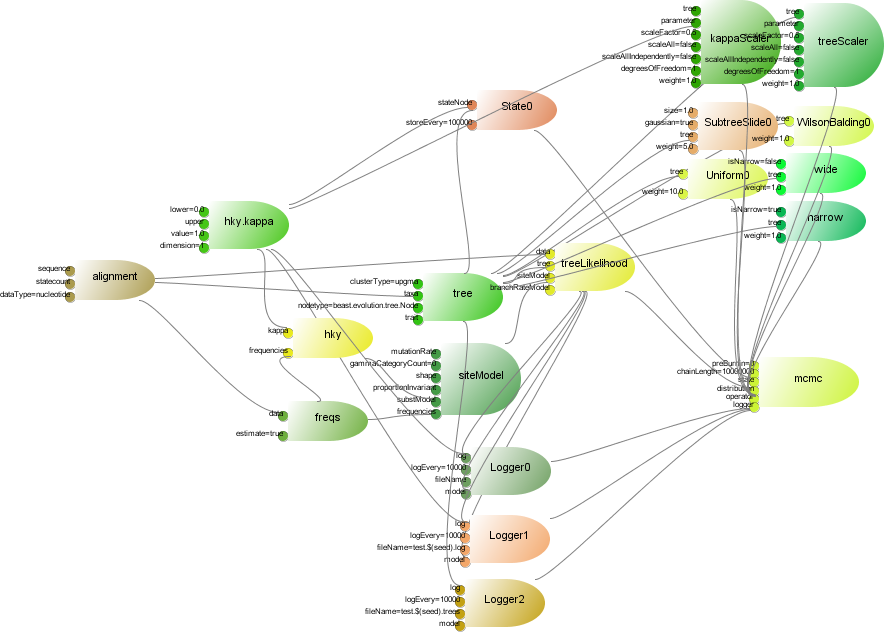
\includegraphics[width=\textwidth]{example5.png}
\figcaption{\label{fig.hky4}Adding the loggers.}\rm\\\hskip10pt
%\end{figure*}

For the MCMC analysis to be any useful, we need to log results. Loggers take care of
this task. Loggers can log anything that is Loggable, such as parameters and trees,
but it is easy enough to write a custom logger and add it to the list of inputs of
a Logger. Typically, one logger logs to standard output, one to a log file with
parameter values (a tab delimited file that can be analysed with Tracer) and one
log file with trees in Newick format.


%\begin{figure*}[h]
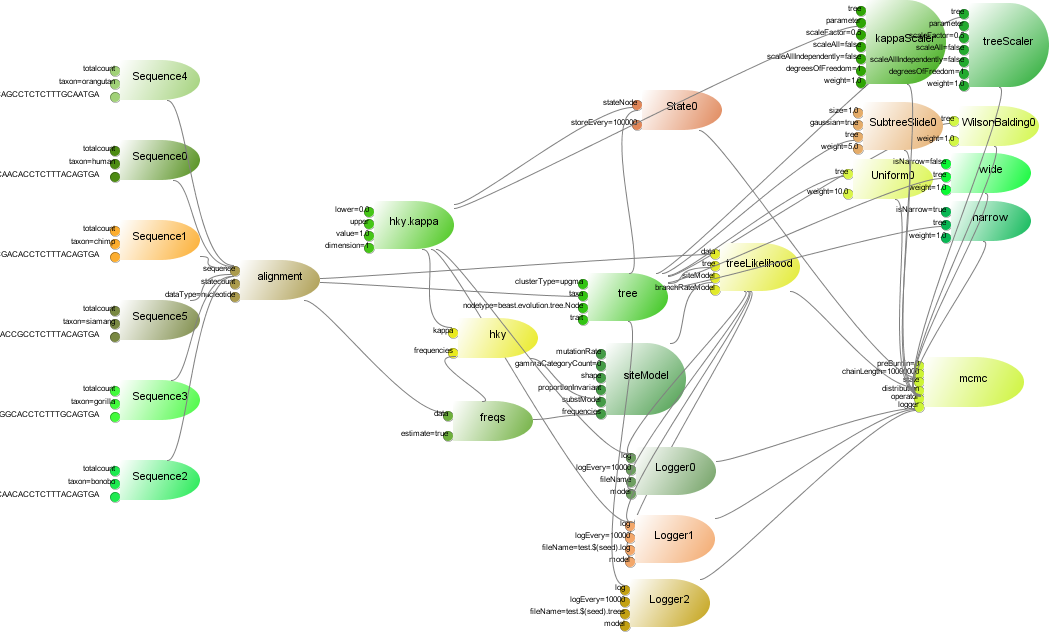
\includegraphics[width=\textwidth]{example6.png}
\figcaption{\label{fig.hky5}Adding the sequences. This is a complete model description
that can be executed in Beast II.}\rm\\\hskip10pt
%\end{figure*}



Finally, the alignment consist of a list of sequences. Each sequence object containing
the actual sequence and taxon information. This completes the model, shown in Figure 
\ref{fig.hky5} and this model can be executed by Beast II.





\section{Getting started\label{sec.start}}


\subsection{Beast II Philosophy}

Everything is a plug-in!

Plug-ins provide...
\begin{itemize}
\item connection with with other plug-ins/values through 'inputs'
\item validation
\item documentation
\item 'XML parsing'
\end{itemize}

The task of a Plugin writer is to create classes, specify inputs and provide 
extra validation that is not already provided by inputs. The following snippet
shows a very basic example.

{\color{blue}\begin{lstlisting}[language=java]
@Description("Description of MyPlugin goes here")
public class MyPlugin extends Plugin {
    public Input<Integer> m_value = new Input<Integer>("value",
        "value used by my plugin");

    public void initAndValidate() throws Exception {
        // go check stuff and 
        // do stuff that normally goes in a constructor
    }

} // class MyPlugin
\end{lstlisting}}

Firstly, the {\tt Description} annotation is used to provide help, which is used in GUIs
online help and documentation generation. There is also a {\tt Citation} annotation
that can be used to list a reference and DOI of a publication that should be
referenced when using the Plugin.

Secondly, all custom Plugins derive from Plugin or any of derived classes from Plugin.
By deriving from Plugin,  services through introspection like validation of models are
provided.

To specify an input for a plugin, just declare an {\tt Input} member. Input is a template
class, so the type of input can be specified to make sure that when Inputs are connected
to Plugins the correct type of Plugin is used. At least two strings are used in the 
constructor of an Input:
\begin{itemize}
\item a name of the input, used in the XML, in documentation and in GUIs,
\item a description of the input, used in documentation and GUI help.
\end{itemize}
Other constructors exists to support validation, default values, lists of values,
enumerations of Strings, etc. See Section \ref{ssec.input} for details.

Finally, there is the {\tt initAndValidate} method. This serves as a place to perform
validation on the Inputs, for instance range checks or check that dimensions of two
inputs are compatible. Furthermore, it is a place to perform everything that normally
goes into a constructor. Plugins are typically created by the XMLParser, which firsts
sets values for all inputs, then calls initAndValidate.

The following shows the skeleton of a bit larger example:

{\color{blue}\begin{lstlisting}[language=java]
@Description("HKY85 (Hasegawa, Kishino & Yano, 1985) "+
        "substitution model of nucleotide evolution.")
@Citation("Hasegawa, M., Kishino, H and Yano, T. 1985. "+
        "Dating the human-ape splitting by a "+ 
        "molecular clock of mitochondrial DNA. " +
        "Journal of Molecular Evolution 22:160-174.")
public final class HKY extends SubstitutionModel.Base {
    public Input<RealParameter> kappa = new Input<RealParameter>("kappa", 
        "kappa parameter in HKY model", Validate.REQUIRED);

    @Override
    public void initAndValidate() throws Exception {
    }

    @Override
    public void getTransitionProbabilities(double distance, double[] matrix) {
        ...
    }

    @Override
    protected boolean requiresRecalculation() {
        ...
    }

    @Override
    protected void store() {
        ...
    }

    @Override
    protected void restore() {
        ...
    }
}
\end{lstlisting}}



\subsection{Inputs\label{ssec.input}}

Inputs can be created that are primitives, plugins, lists or enumerations.
By calling the appropriate constructor, the XMLParser validates the input
after assigning values and can check whether a REQUIRED input is assigned
a value, or whether two inputs that are XOR have exactly one input specified.


\subsubsection{Input creation}
Inputs can be simple primitives, like Double, Integer, Boolean, String.


{\color{blue}\begin{lstlisting}[language=java]
public Input<Boolean> m_pScaleAll = 
    new Input<Boolean>("scaleAll", 
        "if true, all elements of a parameter (not tree) are scaled, otherwise one is randomly selected",
        new Boolean(false));
\end{lstlisting}}

Inputs of a plugin can be other plugins.

{\color{blue}\begin{lstlisting}[language=java]
public Input<Frequencies> m_freqs = 
    new Input<Frequencies>("frequencies", 
        "frequencies nucleotide letters");
\end{lstlisting}}

Inputs can be multiple inputs. When a list of inputs is specified,
the Input constructor should contain a (typically empty) List as a start value.

{\color{blue}\begin{lstlisting}[language=java]
public Input<List<RealParameter>> m_pParameters = 
    new Input<List<RealParameter>>("parameter", 
        "parameter, part of the state",
        new ArrayList<RealParameter>());
\end{lstlisting}}

Inputs cannot be template classes, so {\tt Input<Parameter<T>>} would lead to
trouble. This is due to a limitation in Java introspection.

To provide an enumeration as input, the following constructor can be
used: it takes the usual name and description arguments, then the default
value and an array of strings to choose from. During validation it is 
checked that the value assigned is in the list.

{\color{blue}\begin{lstlisting}[language=java]
	final static String [] UNITS =  {"year", "month", "day"};
	
	public Input<String> m_sUnits = new Input<String>("units", 
            "name of the units in which values are posed, " +
			"used for conversion to a real value. This can be " + 
            Arrays.toString(UNITS) + " (default 'year')", 
            "year", 
            UNITS);
\end{lstlisting}}


\subsubsection{Input validation}

To provide some basic validation, an extra argument can be provided to the Input constructor.
By default, inputs are considered to be OPTIONAL, i.e., need not necessarily be specified.
If input is REQUIRED:

{\color{blue}\begin{lstlisting}[language=java]
public Input<Parameter> m_kappa = 
    new Input<Parameter>("kappa", 
        "kappa parameter in HKY model",
        Validate.REQUIRED);
\end{lstlisting}}

If a list of inputs need to have at least one element specified, the required
argument needs to be provided.

{\color{blue}\begin{lstlisting}[language=java]
public Input<List<Operator>> m_operators = 
    new Input<List<Operator>>("operator",
        "operator for generating proposals in MCMC state space",
        new ArrayList<Operator>(), Validate.REQUIRED);
\end{lstlisting}}

Sometimes either one or another input is required, but not bot. In that case
an input is declared XOR and the {\em other} input is provided as extra argument.
The XOR goes on the second Input.

{\color{blue}\begin{lstlisting}[language=java]
public Input<Tree> m_pTree = 
    new Input<Tree>("tree", 
        "if specified, all tree branch length are scaled");
public Input<Parameter> m_pParameter = 
    new Input<Parameter>("parameter", 
        "if specified, this parameter is scaled"
        , Validate.XOR, m_pTree);
\end{lstlisting}}


\subsection{MCMC library\label{ssec.mcmc}}

The basic setup: The {\tt MCMC} algorithm has a {\tt State} object. {\tt Operator} objects do 
proposals to change the State. A {\tt Distribution} object calculates the posterior of the
new state, and compares it with the old state's posterior (taking the Hasting ration of the
{\tt Operator} in account) to decide whether to accept or reject the new state.

Typically, a plugin developer will create new {\tt CalculationNode}s and {\tt Operator}s,
explained below.

\subsubsection{CalculationNodes\label{ssec.calc}}

A {\tt State} contains {\tt StateNodes}, like {\tt Parameter}s and {\tt Tree}s. The {\tt State}
is responsible for calling {\tt requiresRecalculation}/{\tt store}/{\tt restore} on calculation nodes. It keeps
track which part of the State is changed by an Operation, hence which {\tt CalculationNode}s
may need updating.

For example, suppose a scale operator (called kappScaler) changes the kappa parameter in
a simple HKY model. Then, frequencies, and the tree are not affected, but the substitution
model, the site model and the tree likelihood need to be updated.

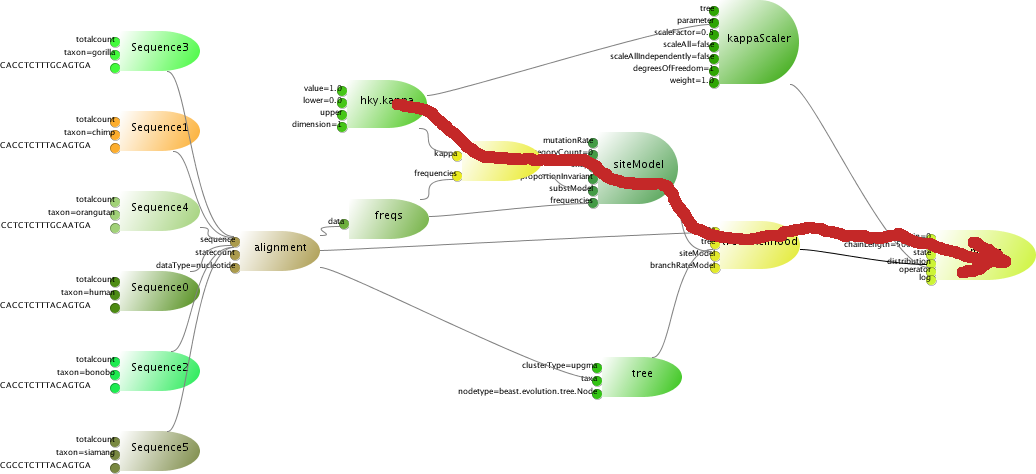
\includegraphics[width=\textwidth]{hky.png}

After an {\tt Operator} has done a proposal, the {\tt State} calls {\tt store} on all {\tt CalculationNode}s
that could possibly be affected.
Then State calls {\tt requiresRecalculation} on each of the 
{\tt CalculationNode}s between the {\tt StateNode}s that are changed and the {\tt Distribution} of the {\tt MCMC}.
The {\tt requiresRecalculation} method returns true to indicate whether the CalculationNode
is changed, hence is 'dirty', due to changes in the State. Also, it is a good place to set
flags whether parts need to be recalculated, e.g. the EigenDecomposition in the HKY model
after the kappa parameter is changed.
Then, the distribution is asked to calculated the log-posterior. If the new state is
accepted, {\tt accept} is called on all {\tt CalculationNode}s, which by default just marks
them as 'not dirty'. If rejected, a {\tt restore} is called on all {\tt CalculationNode}s
and this method can be overridden to 


In summary: typically a Plugin developer overrides a {\tt CalculationNode}.

{\tt CalculationNode}s can help increase efficiency by overwriting
\begin{itemize}
\item {\tt requiresRecalculation} to set flags to recalculate parts and return
whether the Plugin is dirty or not.
\item {\tt store} to store internal states.
\item {\tt restore} to restore when a new State is not accepted.
\end{itemize}

\subsubsection{Operators\label{ssec.oper}}

{\tt Operator}s need to have at least one {\tt StateNode} as input.
{\tt StateNode}s are managed by the {\tt State}, which takes care of synchronization,
store and restore.

To create a new Operator, implement the {\tt public double proposal()} method, 
which changes one of more {\tt StateNode}s and returns the Hasting ratio of the proposal.

\begin{center}{\huge WARNING}\end{center}

When retrieving a {\tt StateNode} to operate on, use {\tt Input.get(this)} instead of
{\tt Input.get()}. 

The latter will {\em not} notify the {\tt State} and changes can be lost or not
propagate through at all.

\subsubsection{Loggable\label{ssec.logger}}

To create custom loggers, implement the {\tt Loggable} interface, which has three methods:\\
o init(), for generating header information and called only at the start of the log,\\
o exit(), for any closing statements, e.g. 'End;' in a Nexus tree file, and\\
o log(), for periodically logging relevant information.



\subsection{Evolution library\label{ssec.evo}}

The Evolution library provides support for calculating posteriors for
phylogenetic analysis. The classes of interest are
\begin{itemize}
\item{\em SubstitutionModel} Specifies transition probability matrix for a given distance.
\item{\em BranchRateModel} Defines a mean rate for each branch in the beast.tree.
\item{\em SpeciationLikelihood} A likelihood function for speciation processes.
\item{\em tree.Node} Nodes in building binary beast.tree data structure.
\item{\em PopulationFunction} A population size function for the Coalescent.
\end{itemize}

See javadocs for details.


\section{XML format\label{sec.xml}}

The easiest way to create XML for a newly created Plugin is to start the ModelBuilder
({\tt java -cp beast.jar beast.app.ModelBuilder}), load an existing XML file
from the example directory and change the Plugins, then save the XML.

The basic XML is very very simple: everything can be specified using
the {\tt input} element. There are 4 reserved attributes, namely id, idref, 
name and spec.

\begin{verbatim}<input id='myId'
     idref='otherId'
     name='inputName'
     spec='x.y.z.MyClass'  />
\end{verbatim}

The id attribute allows elements to be referred to from other elements through
the idref attribute. The name attribute specified the name of the Input in the
plugin. The spec attribute specifies the Plugin class. The XML parser creates
an object of this class, then set the input with name {\tt name} of the Plugin
specified by the enclosing input element. This way every model can be 
specified, but it is very tedious format to read. So, there are a lot of 
short cuts, making the XML more palatable.

A hand crafted XML file can be processed through the XMLParser as follows:
{\tt java -cp beast.jar beast.util.XMLParser <file.xml>} which then 
tries to beautify the XML and print it to standard output.

\subsection{Short XML spec}
The following elements are reserved keywords:
distribution, operator, logger, data, sequence, state, parameter, tree, and run
which have default mappings to objects.
Furthermore, {\tt <plate var='n' range='.p1,.p2,.p3'><parameter idref='hky\$(n)'/></plate>}
is short for 
{\tt <parameter idref='hky.p1'/>
<parameter idref='hky.p2'/>
<parameter idref='hky.p3'/>}
and the top level element should have attribute {\tt version='2.0'}
and can have {\tt namespace='x.y.z:'} which allows {\tt spec}-attributes
to use {\tt x.y.z} as name space. Finally, {\tt <map name='elementName'>x.y.z.Class</map>}
maps element {\tt elementName} to spec {\tt x.y.z.Class}.

Common abbreviations:


Element name = name attribute.

{\color{blue}\tt <input name='x'>...</input> == <x> ... </x>}

Primitive inputs (Integer, Double, Boolean, String) can go inline.

{\color{blue}\tt <input ...> <input name='xyz' value='1.0'/></input> 

== 

<input ... xyz='1.0'/>}

Any plugin with String constructor, like parameters and tree, can go inline

{\color{blue}\tt <input ...> <xyz spec='IntegerParameter' value='10 20'/></input> 

== 

<input ... xyz='10 20'/>}

Idref inline using @ sign.

{\color{blue}\tt <input ...> <input name='xyz' idref='ref'/></input> 

== 

<input ... xyz='@ref'/>}





%\subsection{Resolving name}
%\subsection{Resolving class}
%\subsection{Resolving idref}
%\subsection{Plates}





\section{FAQ/Known ways to get into trouble\label{sec.faq}}

\subsubsection{{\tt Input} is not declared public.}

If {\tt Input}s are not public, they cannot get values assigned by for
instance the {\tt XMLParser}.

\subsubsection{{\tt Operator} calls {\tt input.get()} instead of {\tt input.get(this)}.}

When an {\tt Operator} does a proposal, it should change a {\tt StateNode}.
This {\tt StateNode} needs to be one of its inputs. So, to get the {\tt StateNode}
normally a call to {\tt input.get()} would give the value. However, for the
{\tt State} to know that a {\tt StateNode} changes, the method {\tt input.get(this);}
should be called.

Note that this only applies to the {\tt proposal()} method, not to {\tt initAndValidate()}
(though it does not hurt in the latter) since only in {\tt proposal()} a {\tt StateNode}
should be changed.

\subsubsection{Shadow a {\tt StateNode} in a {\tt CalculationNode}.}

It is tempting to use a pattern like this:

{\color{blue}\begin{lstlisting}[language=java]
public Input<RealParamater> m_p = new Input<>...;
    private RealParameter m_pShadow;

    public void initAndValidate() {
        m_pShadow = m_p.get();
    }
    
    double calculateSomethingOld() {
        // uses non-current value
        return m_pShadow.getValue() * 2.0;
    }

    double calculateSomethingNew() {
        // uses current value
        return m_p.get().getValue() * 2.0;
    }
\end{lstlisting}}

in a Plugin. However, {\tt StateNode}s like {\tt RealParameter} can change their
value and the {\tt m\_p.get()} may return a different object next time it is called.
So, the method {\tt calculateSomethingOld()} above may return the same initial value
every time, while {\tt calculateSomethingNew()} above uses the current values of
parameter {\tt m\_p} and follows the changes of {\tt m\_p} when it changes in the State.

To ensure always a current version of the {\tt StateNode} is available, call
{\tt get()} every time at the start of a method.


\subsubsection{Type of input is a template class (other than {\tt List}).}

Thanks to limitations of Java introspection and the way Beast II is set up, Inputs should be 
of a type that is concrete, and apart from {\tt List<T>} no template class should be used.

\subsubsection{Store/restore do not call {\tt super.store()}/{\tt super.restore()}.}

Obviously, not calling store/restore on super classes may result in unexpected behavior.

\subsubsection{Input rule of base class is not what you want.}

If an Input is REQUIRED for a base class you want to override, but for the derived
class this Input should be OPTIONAL, set the Input to OPTIONAL in the constructor.
E.g. for a SNPSequence that derives from Sequence, but for which m\_sData is optional,
add a constructor

{\color{blue}\begin{lstlisting}[language=java]
	public SNPSequence() {
		m_sData.setRule(Validate.OPTIONAL);
	}
\end{lstlisting}}
Note that the constructor needs to be public, to prevent IllegalAccessExceptions
on construction by e.g. the XMLParser.


\end{document}


